%%%
%
% $Autor: Wings $
% %Projekt: 
% $Datum: 2025-06 $
% Dateiname: SensorHCSR04.tex
%
% !TeX spellcheck = de_DE/GB
% !TeX program = pdflatex
% !BIB program = biber/bibtex
% !TeX encoding = utf8
%
%%%

\chapter{Ultraschall-Abstandssensor HC-SR04}\label{HCSR04}

%Einleitung
%\Mynote{cite books, applications, board}

\subsection{Einleitung}

Im folgenden Abschnitt wird der Ultraschall-Abstandssensor HC-SR04 betrachtet. Dazu zählen seine physikalischen Grundlagen, seine Funktionsweise und Anwendungsbeispiele aus Industrie, Automation und Medizin.

\subsection{Grundlagen zur Verwendung eines Ultraschall-Abstandssensors}\label{GrundlagenVerwendungAbstandssensor}

\subsubsection{Grundlagen Schall}

Als Schall bezeichnet man die Ausbreitung von lokalen Druckschwankungen in einem elastischen Medium. Die Schallwelle breitet sich dabei longitudinal aus, die Auslenkung der Moleküle erfolgt also in Ausbreitungsrichtung \cite{Kersten:2024}.
Die Einteilung der Schallbereiche erfolgt auf Grundlage der Frequenz:

\begin{itemize}
    \item \textit{Infraschall:} bis 16 Hz,
    \item \textit{Hörbarer Schall:} von 16 Hz bis 20 kHz,
    \item \textit{Ultraschall:} von 20 kHz bis 1 GHz,
    \item \textit{Hyperschall:} über 1 GHz \cite{Hering:2023}.
\end{itemize}

In Abbildung \ref{fig:Schallwellen} werden die Schallwellen von Infraschall, Schall und Ultraschall dargestellt.

\begin{figure}[!ht]
	\centering
	\resizebox{1\textwidth}{!}{%
		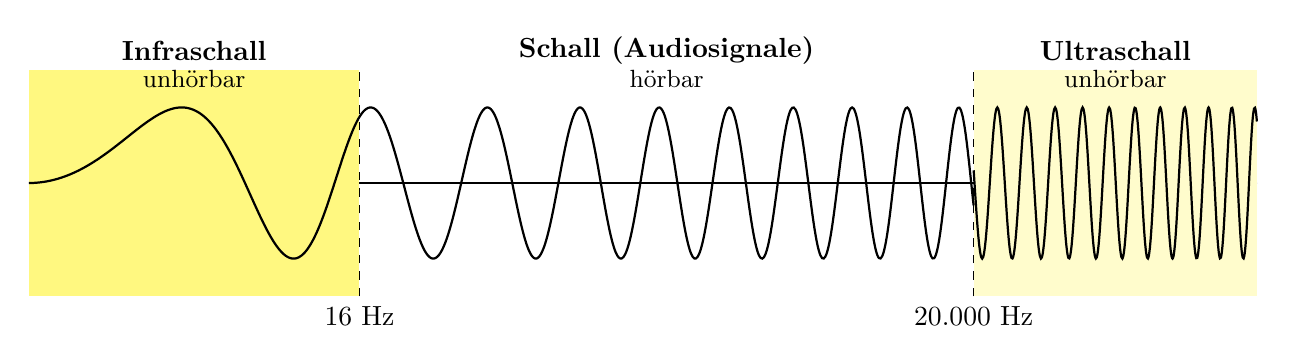
\begin{tikzpicture}[scale=1.2]
			% Achse
			\draw[->] (0,0) -- (13,0) node[right] {};
			
			% Bereichsfarben
			\fill[yellow!50] (0,-1.2) rectangle (3.5,1.2);   %Infraschall
			\fill[yellow!20] (10,-1.2) rectangle (13,1.2);   %Ultraschall
			
			% Beschriftungen
			\node at (1.75,1.4) {\textbf{Infraschall}};
			\node at (1.75,1.1) {\small unhörbar};
			
			\node at (6.75,1.4) {\textbf{Schall (Audiosignale)}};
			\node at (6.75,1.1) {\small hörbar};
			
			\node at (11.5,1.4) {\textbf{Ultraschall}};
			\node at (11.5,1.1) {\small unhörbar};
			
			% Frequenzgrenzen
			\draw[dashed] (3.5,-1.2) -- (3.5,1.2);
			\node[below] at (3.5, -1.2) {16 Hz};
			
			\draw[dashed] (10,-1.2) -- (10,1.2);
			\node[below] at (10, -1.2) {20.000 Hz};
			
			% Schallwelle (stückweise)
			\draw[thick, domain=0:10, samples=600, smooth, variable=\x] 
			plot ({\x}, {0.8*sin(deg(0.6*\x*\x))});
			
			\draw[thick, domain=10:13, samples=300, smooth, variable=\x] 
			plot ({\x}, {0.8*cos(deg(1.2*(\x-2)*(\x-2)))});  % Höhere Frequenz im Ultraschallbereich
			
		\end{tikzpicture}
	}%
	\caption{Schallwellen}
	\label{fig:Schallwellen}
\end{figure}

\Ausblenden{
\begin{center}
	
\includegraphics[width=5in]{Sensor/HCSR04/Schall}
	\captionof{figure}{Infraschall, Hörbarer Schall, Ultraschall}
	\label{Schallgrafik}
\end{center}
}

\subsubsection{Schallgeschwindigkeit und Wellenlänge}\label{AbschnittVschall}

Die Geschwindigkeit, mit der sich Schall in Luft ausbreitet, ist von der Lufttemperatur $T$ und der Luftfeuchtigkeit $\varphi$ abhängig. Da die Luftfeuchtigkeit einen erheblich geringeren Einfluss auf den Wert hat \ref{Vphi}

\begin{equation}
    \Delta v_{Schall,\varphi}\approx1,2\:\dfrac{\text{m}}{\text{s}}; \:0<\varphi<1, \:T_{C}=20 \:\text{\textcelsius},
    \label{Vphi}
\end{equation}

\cite{Hering:2023} lässt sich die Schallgeschwindigkeit mit ausreichender Genauigkeit mit der Formel \ref{Vschall}

\begin{equation}
    v_{Schall}=\sqrt{\kappa R T}
    \label{Vschall}
\end{equation} 

und der Annahme $\varphi=0$ berechnen \cite{Tipler:2024}. 
Dabei ist $\kappa = 1{,}4$ der Adiabatenexponent von Luft, $R=287$ \(\dfrac{\text{J}}{\text{kg K}}\) die spezifische Gaskonstante von Luft und $T$ die absolute Temperatur in Kelvin \cite{Tipler:2024,Willems:2022}.
Für eine angenommene Temperatur von $T_{C} = 20\:\text{\textcelsius}$ ergibt sich damit eine Geschwindigkeit von $v_{Schall}=343,2\:\dfrac{\text{m}}{\text{s}}$.


In Abbildung \ref{schallfunktion} ist die Schallgeschwindigkeit in Luft im Temperaturbereich von $T_{C} = -10 \:\text{\textcelsius \:bis } \:60 \:\text{\textcelsius}$ dargestellt.

\begin{figure}[h]
    \begin{center}
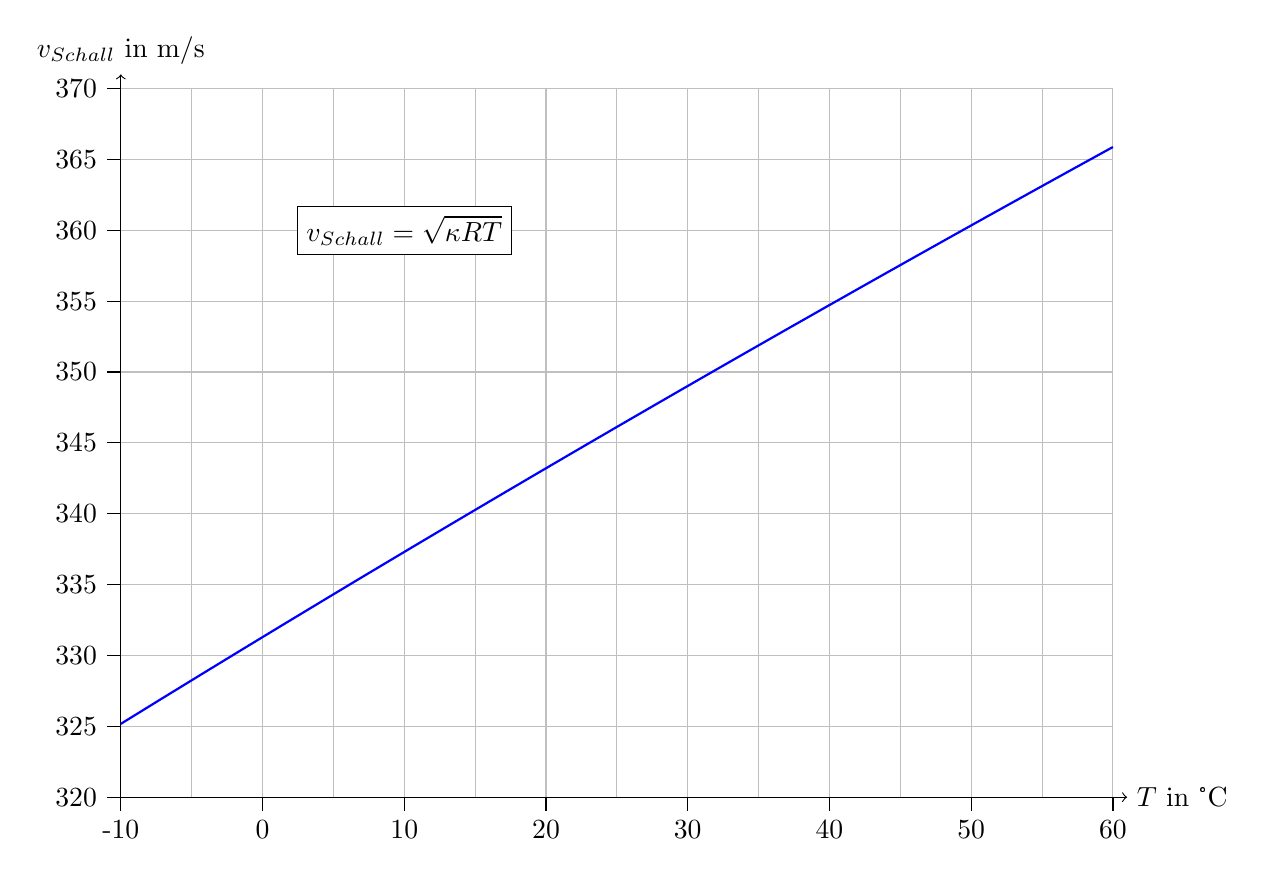
\begin{tikzpicture}
    \begin{scope}[scale=.9]
        %Gitter im Hintergrund
        \draw[lightgray] (-2,4) grid (12,14); 
        
        %Achsen
        \draw[thin, ->] (-2,4) -- (12.2,4) node[right] {$T$ in °C}; %x-Achse
        \draw[thin, ->] (-2,4) -- (-2,14.2) node[above] {$v_{Schall}$ in m/s}; %y-Achse
        %Beschriftung
        \foreach[count=\x] \a in {-10, 0, 10, 20, 30, 40, 50, 60} {
            \draw[thin] (2*\x-4,4) -- (2*\x-4,3.8) node [below] {\a};
        }%x-Achse
        \foreach[count=\x] \a in {320, 325, ..., 370} {
            \draw[thin] (-2,\x+3) -- (-2.2,\x+3) node [left] {\a};
        }%y-Achse
        
        %Funktion
        \draw[scale=2, thick, domain=26.316:33.316, variable=\T, blue] plot ({\T-27.316}, {sqrt(\T*40.18)-30});
        \node at(2,12) [rectangle,fill=white, draw] {$v_{Schall}=\sqrt{\kappa R T}$};
        
        %Vergleichsfunktion
        %\draw[gray] plot coordinates {(-2,5) (12,13.2)};
    \end{scope}
\end{tikzpicture}        \caption{Ausbreitungsgeschwindigkeit von Schall in Luft}
        \label{schallfunktion}
    \end{center}
\end{figure}

Über den Formelzusammenhang \ref{Wellenlaenge}

\begin{equation}
    v_{Schall}=\lambda f
    \label{Wellenlaenge}
\end{equation}

lässt sich bei gegebener Frequenz $f$ und mit der berechneten Schallgeschwindigkeit $v_{Schall}$ die Wellenlänge $\lambda$ des Schalls berechnen \cite{Willems:2022}. Diese beträgt bei einer angenommenen Frequenz von $f=40 \:\text{kHz}$ und der in Abschnitt \ref{AbschnittVschall} berechneten Schallgeschwindigkeit $\lambda=8{,}58\cdot10^{-3} \:\text{m}$.

\subsubsection{Absorption und Reflexion}

Absorption beschreibt die Abnahme der Intensität $I$ einer Schallwelle, während sie einen Weg durch das sie leitenden Medium zurücklegt. Sie ist vom Quadrat der Frequenz $f$ des Schalls und den Absorptionseigenschaften $a$ des Ausbreitungsmediums abhängig und lässt sich über die Formel \ref{Absorption}

\begin{equation}
    I(x)=I_0\times\exp(-\alpha x); \:\alpha=af^2
    \label{Absorption}
\end{equation}

berechnen \cite{Hering:2023,Hering:2021b}.
In Abbildung~\ref{DiagrammIntensitaet} ist die Abhängigkeit des Verhältnisses der Intensität $I$ zu $I_0$ von der Frequenz dargestellt. Die Wegstrecke von einem Meter und die Umgebungsbedingungen sind entsprechend konstant.

Für eine Frequenz von $f=40 \:\text{kHz}$ ergibt sich ein Verhältnis von 0,95.

\begin{figure}[h]
    \begin{center}
%Diagramm Intensität
%Abstandssensor\Entwicklerdokumentation\tikz
%tikz-Diagramm für die Abhängigkeit der Intensität von der Frequenz (qualitativ)
%Bestandteil der Entwicklerdokumentation "Abstandssensor" (Automatisierungstechnik SS24)

\begin{tikzpicture}
    \begin{scope}[scale=.85]	
        %Achsen
        \draw[thin, ->] (0,0) -- (10.2,0) node[right] {$f$ in KHz}; %x-Achse
        \draw[thin, ->] (0,0) -- (0,8.2) node[above] {$I/I_0$}; %y-Achse
        %Beschriftung
        \foreach[count=\x] \a in {0, 20, ..., 200} {
            \draw[thin] (\x-1,0) -- (\x-1,-0.2) node [below] {\a};
        }%x-Achse
        \foreach[count=\x] \a in {0.0001, 0.0010, 0.0100, 0.1000, 1.0000} {
            \draw[thin] (0,\x*2-2) -- (-0.2,\x*2-2) node [left] {\a};
        }%y-Achse
        
        %Funktion, qualitativ!
        \draw[thick, domain=0:10, variable=\x, blue] plot ({\x}, {-0.0741*\x^2+8});
    \end{scope}
\end{tikzpicture}
        \caption{Abnahme der Schallintensität in Abhängigkeit der Frequenz bei einem Meter, nach \cite{Hering:2023}}
        \label{DiagrammIntensitaet}
    \end{center}
\end{figure}

Trifft die Schallwelle auf die Grenzschicht zweier Medien mit verschiedenen Schallkennimpedanzen $Z_n$, wird sie zum Teil reflektiert und zum anderen Teil transmittiert. Der Reflexionsgrad ist bei großen Differenzen zwischen den Impedanzen $\left(Z_1 \ll Z_2 \:\text{oder} \:Z_1 \gg Z_2\right)$ der Medien besonders hoch. Sind die Impedanzen hingegen ähnlich $\left(Z_1 \approx Z_2\right)$ ist der Absorptionsgrad sehr hoch \cite{Hering:2021b}. 
Da viele Flüssigkeiten und feste Stoffe eine um den Faktor $10^4 \:\text{bis} \:10^5$ höhere Impedanz im Vergleich zu Luft vorweisen, ist der Reflexionsgrad in diesen Fällen $\gg 99\%$ \cite{Hering:2021b,Hering:2023}.

\subsubsection{Weg- und Abstandsmessung mit Ultraschall}

Um eine Entfernung oder einen Abstand eines Objekts zu dem Sensor zu ermitteln, wird der Sensor im sog. Tastbetrieb mit Echo-Laufzeit-Messung, wie in Abbildung \ref{TastbetriebELM} zu sehen, verwendet. Dabei sendet der Sensor über den integrierten Lautsprecher zunächst einen Schallpuls in Richtung des zu messenden Objekts aus, welcher zum Teil von dem Objekt reflektiert wird und als Echo zurück zum Sensor gelangt. Dieses Echo kann der Sensor über das integrierte Mikrofon detektieren und über die gemessene Laufzeit des Echos sowie der Schallgeschwindigkeit im Medium, welches den Sensor umgibt, die Distanz berechnen \cite{Hering:2023}. Dies ist sowohl in gasförmigen Medien, als auch in flüssigen Medien der Fall.

\begin{figure}[h]
    \begin{center}
%Funktionsweise
%Abstandssensor\Entwicklerdokumentation\tikz
%tikz-Diagramm zur Funktionsweise eines Ultraschallsensors (qualitativ)
%Bestandteil der Entwicklerdokumentation "Abstandssensor" (Automatisierungstechnik SS24)

\begin{tikzpicture}
    %Achsen
    \draw[thin, ->] (0,0) -- (10.2,0) node[right] {$t$}; %x-Achse
    \draw[thin, ->] (0,0) -- (0,4.2) node[above] {$U$}; %y-Achse
    
    %Funktion, qualitativ!
    \draw[thick, blue] plot [smooth] coordinates{(1,0) (2,3) (4,3.5) (4.5,1) (5,0.1) (6,0)};
    \draw[thick, blue] plot [smooth] coordinates{(8,0) (8.3,0.1) (9,0.8) (9.7,0.1) (10,0)};
    
    %Beschriftung
    \node at (1,0) [anchor=south east] {$t_0$};
    \node at (8,0) [anchor=south east] {$t_1$};
    \draw[dotted] (4.5,1) -- (5,2) node[anchor=south west]{Sendeimpuls}; 
    \draw[dotted] (9,0.8) -- (9.5,2) node[anchor=south]{Echo}; 
    \draw (1,0) -- (1,-2.2);
    \draw (8,0) -- (8,-2.2);
    \draw[<->] (1,-2) -- (4.5,-2) node[anchor=south]{Echolaufzeit} -- (8,-2);
    \draw (4,0) -- (4,-1.2); 
    \draw (6,0) -- (6,-1.2); 
    \draw[<->] (1,-1) -- (2.5,-1) node[anchor=south]{$\delta t$} -- (4,-1);
    \draw[<->] (4,-1) -- (5,-1) node[anchor=south]{\tiny{Ausschwingzeit}} -- (6,-1);
\end{tikzpicture}
        \caption{Spannungsverlauf Schallwandler bei einer Echo-Laufzeit-Messung, nach \cite{Hering:2023}}
        \label{TastbetriebELM}
    \end{center}
\end{figure}

Bei der Anwendung einköpfiger Sensoren ist bei der Messung sehr kleiner Distanzen auf die Ausschwingzeit des Wandlers sowie auf die Umschaltzeit vom Lautsprecher- in den Mikrofonbetrieb zu achten, da während dieser Zeit kein Echosignal aufgenommen werden kann. Daraus folgt eine geringere Abtastfrequenz als bei zweiköpfigen Ultraschall-Abstandssensoren. Bei zweiköpfigen Ultraschall-Abstandssensoren, also je einem dedizierten Lautsprecher und einem Mikrofon, sind die Öffnungswinkel der Schallkeulen in Verbindung mit dem radialen Abstand maßgeblich für die minimale Distanz.  

Bei großen Distanzen sind sowohl die Genauigkeit der Ausrichtung des Sensors als auch die Absorption der Schallintensität in dem Ausbreitungsmedium relevant \cite{Hering:2023}. 

Ebenfalls störend können sich die Geometrie des zu messenden Objektes $\left(\text{z. B. bei stark konkaven oder konvexen Oberflächen}\right)$, absorbierendes/diffus reflektierendes Material $\left(\text{Filz, Watte, Schaumstoff}\right)$ oder Umwelteinflüsse orthogonal zur Messrichtung wirkender Wind auswirken. Verunreinigungen wie Staub und Rauch oder leichter Niederschlag in Form von Regen und Schnee beeinträchtigen die Messung hingegen nicht \cite{Hering:2023}.


\subsubsection{Herausforderungen}

Dadurch, dass die Schallgeschwindigkeit von der Umgebungstemperatur abhängig ist, muss diese für die Berechnung der Distanz mit einbezogen werden, wenn der Sensor in einem größeren Temperaturbereich eingesetzt werden soll. In Abbildung~\ref{schallfunktion} ist zu erkennen, dass die Differenz der Geschwindigkeit in dem Temperaturbereich, in dem alle Komponenten des Sensors betrieben werden könnten $\left(-10 \:\text{\textcelsius}\leq T_{C}\leq55 \:\text{\textcelsius}\right)$, etwa $38 \:\dfrac{\text{m}}{\text{s}}$ beträgt. Dies entspricht, ausgehend von dem Standardwert für die Schallgeschwindigkeit $v_{Schall,20}=343,2\:\dfrac{\text{m}}{\text{s}}$, einer Streuung von $-5,2\% \:\text{und} \:+5,8\%$. Hinzu kommt die Unsicherheit aufgrund der Luftfeuchtigkeit. Hier liegt die Streuung, bezogen auf die Schallgeschwindigkeiten bei $\varphi=0$, in einem Bereich zwischen $+0,37\% \:\text{für} \:T_{C}=-10\:\text{\textcelsius} \:\text{und} \:+0,33\% \:\text{für} \:T_{C}=55 \:\text{\textcelsius}$.

Physikalische Effekte wie die Absorption, welche unter Laborbedingungen maßgeblich die Reichweite des Sensors einschränken, oder einen schlechten Reflexionsgrad bestimmter Materialien, schränken das System in seiner Vielseitigkeit ein. Selbiges gilt für Attribute des Sensors wie die Ausschwingzeit des Schallwandlers oder die geometrische Anordnung der Schallkeulen bei zweiköpfigen Systemen.
Auch die genannten Umwelteinflüsse können dafür sorgen, dass eine Messung fehlschlägt oder ein falsche Ergebnis liefert \cite{ifm:2025}.

\subsubsection{Anwendungsbeispiele}
Ultraschall-Abstandssensoren finden in zahlreichen Bereichen Anwendung, in denen eine berührungslose und verschleißfreie Messung unabhängig von Farbe, Transparenz oder Oberflächenbeschaffenheit erforderlich ist. Dies macht sie besonders geeignet für den Einsatz in der Automatisierungstechnik, der Medizintechnik sowie in industriellen Prozessen \cite{Conrad:2024,Smoot:2021}.

Basierend auf dem Ausbreitungsmedium des Schalls lassen sich Ultraschall-Abstandssensoren in drei Hauptkategorien einteilen \cite{Hering:2023}:

\begin{itemize}
	\item \textbf{Luftschall-Sensoren:} Diese werden typischerweise für Anwendungen wie Füllstandsmessungen, die Durchmessererfassung bei Auf- und Abwickelsteuerungen oder zur Objekterkennung und Kollisionsvermeidung eingesetzt.
	
	\item \textbf{Flüssigkeitsschall-Sensoren:} Hier breitet sich der Schall in flüssigen Medien aus. Solche Sensoren kommen hauptsächlich im maritimen Bereich zum Einsatz, etwa in Sonarsystemen zur Ortung von Unterseebooten oder Fischschwärmen sowie in Echoloten zur Kartografie des Meeresbodens \cite{Hering:2021b}.
	
	\item \textbf{Körperschall-Sensoren:} Diese Kategorie nutzt die Schallausbreitung in festen Materialien. In der Industrie dienen sie häufig zur zerstörungsfreien Werkstoffprüfung. In der Medizin wird die Ultraschalldiagnostik zur bildgebenden Untersuchung von Organen und Föten eingesetzt \cite{Hering:2021b}.
\end{itemize}

Trotz der vielseitigen Einsatzmöglichkeiten müssen bei der Verwendung von Ultraschall-Abstandssensoren gewisse Einschränkungen beachtet werden. Die Messgenauigkeit kann durch schwankende Umgebungsbedingungen wie Temperatur oder Luftfeuchtigkeit beeinträchtigt werden \cite{ifm:2025}.

\subsection{Ultraschall-Abstandsensor HC-SR04}

Der Ultraschall-Abstandssensor in Abbildung~\ref{Ultraschall-Abstandssensor} vom Hersteller JOY-it enthält den Sensor HC-SR04 und ist zur Erfassung von Abständen in einem Bereich von 3 bis 400 cm spezifiziert. Dafür nutzt er eine Schallfrequenz von 40 kHz. Damit führt der Ultraschall-Abstandssensor HC-SR04 jede Sekunde 10-16 Messungen durch. Er ist als zweiköpfiger Sensor ausgeführt, wodurch er über je einen Lautsprecher- und ein Mikrofonkopf verfügt.  Die Abmessungen des Ultraschall-Abstandssensors betragen in der Breite 43 mm, in der Höhe 15 mm und in der Tiefe 20 mm. Die Auflösung des Sensors beträgt $\pm 1$ mm.

    \begin{center}
        
\includegraphics[width=3in]{Sensor/HCSR04/HCSR04}
        \captionof{figure}{Ultraschall-Abstandssensor HC-SR04 der Marke JOY-IT\cite{Simac:2017}}
        \label{Ultraschall-Abstandssensor}
    \end{center}

\begin{figure}[!ht]
	\centering
	\resizebox{1\textwidth}{!}{%
		\definecolor{deepblue}{RGB}{0,0,128}
		\begin{tikzpicture}
			\tikzstyle{every node}=[font=\LARGE]
			\draw[blue, fill=deepblue]  (-7.5,19) rectangle (15.75,9);
			\draw[gray, fill=gray]  (-1.75,14) circle (3.75cm);
			\draw[gray, fill=gray]  (10,14) circle (3.75cm);
			\draw[white, fill=white]  (-6.75,18.25) circle (0.5cm);
			\draw[white, fill=white]  (15,9.75) circle (0.5cm);
			\draw[white, fill=white]  (15,18.25) circle (0.5cm);
			\draw[white, fill=white]  (-6.75,9.75) circle (0.5cm);
			\draw[gray, fill=gray]  (4.25,17.75) ellipse (2.25cm and 0.5cm);
			\draw[gray, fill=gray]  (4.5,9) rectangle (4.75,6.25);
			\draw[gray, fill=gray]  (5.25,9) rectangle (5.5,6.25);
			\draw[gray, fill=gray]  (3.5,9) rectangle (3.75,6.25);
			\draw[gray, fill=gray]  (3,9) rectangle (2.75,6.25);
			\draw[red, fill=red]  (3.75,9.5) circle (0.25cm);
			\draw[blue, fill=blue]  (3,9.5) circle (0.25cm);
			\draw[green, fill=green]  (4.5,9.5) circle (0.25cm);
			\draw[black, fill=black] (5.25,9.5) circle (0.25cm);
			\draw[black!60, fill=black!60]  (10,14) circle (3cm);
			\draw[black!60, fill=black!60]  (-1.75,14) circle (3cm);
			\node [text=white, font=\huge] at (-5.5,10) {T};
			\node [text=white, font=\huge] at (13.5,10) {R};
			\node [text=white, font=\Huge] at (4.25,15.75) {HC-SRO4};
			\node [text=white, font=\LARGE, rotate around={90:(0,0)}] at (3,10.75) {Vcc};
			\node [text=white, font=\LARGE, rotate around={90:(0,0)}] at (3.75,10.75) {Trig};
			\node [text=white, font=\LARGE, rotate around={90:(0,0)}] at (4.5,10.75) {Echo};
			\node [text=white, font=\LARGE, rotate around={90:(0,0)}] at (5.25,10.75) {Gnd};
		\end{tikzpicture}
	}%
	\caption{Ultraschall-Abstandssensor HC-SR04}
	\label{fig:Ultraschall-Abstandssensor1}
\end{figure}

\subsection{Anschlüsse des Ultraschall-Abstandssensors HC-SR04} 
 
 Angeschlossen wird der Abstandssensor über den \ac{scl}-Pin für das Triggersignal, den \ac{sda}-Pin fürs Echo, den \ac{vcc}-Pin zur Stromversorgung und dem \ac{gnd}-Pin \ref{Ultraschall-Abstandssensor}. 
 
 Der Sensor kann über die drei Schnittstellen \ac{gpio}, \ac{uart} und \ac{i2c} verbunden werden \cite{Simac:2017}. In diesem Projekt wird ausschließlich die \ac{i2c}-Schnittstelle genutzt, da sie durch ihren Zwei-Draht-Bus (SDA/SCL) platzsparende Verdrahtung ermöglicht, Störemissionen reduziert und die Synchronisation mehrerer Sensoren vereinfacht \cite{Lee:2018}.


Bei den folgenden Beispielprogrammen wird der Arduino Nano 33 BLE Sense Lite verwendet. In den Beispielen werden die Pins D6/D3 für den Trigger und D9/D2 für das Echo zur Datenübertragung verwendet. In der Tabelle~\ref{PinBelegungUltraschall}  ist dies für die Grove-Schnittstelle festgehalten.

\begin{table}[h]
	\centering
	\renewcommand{\arraystretch}{1.5} % Erhöht den Zeilenabstand für bessere Lesbarkeit
	\setlength{\tabcolsep}{10pt} % Fügt etwas mehr Abstand zwischen den Spalten hinzu
	\caption{Pin Belegung Ultraschall-Abstandssensor HC-SR04}
	\label{PinBelegungUltraschall}
	\begin{tabular}{|m{4cm}|m{6cm}|}
		\hline 
		\rowcolor{black!12}\textbf{Arduino Pin} & \textbf{Ultraschall Abstandssensor} \\ \hline
		\textbf{D9/D2} & Trig \\ \hline
		\textbf{D6/D3} & Echo \\ \hline
		\textbf{\SI{3.3}{\volt}} & \acs{vcc} \\ \hline
		\textbf{GND} & \acs{gnd} \\ \hline
	\end{tabular}
\end{table}

Zu beachten ist jedoch in Benutzung mit dem Arduino Nano 33 BLE Sense Lite, dass der Ultraschall-Abstandssensor HC-SR04 standardmäßig eine Spannung von \SI{5}{\volt} ausgibt, daher besteht beim direkten Anschluss an den Arduino Nano 33 BLE Sense Lite die Gefahr einer Beschädigung des Mikrocontrollers. Der verwendete Mikrocontroller nRF52840 arbeitet ausschließlich mit \SI{3.3}{\volt} - Logikpegeln und ist nicht \SI{5}{\volt} - tolerant \cite{Simac:2017}.

Um diese potenziell schädliche Spannung sicher auf ein kompatibles Niveau zu bringen, wird ein Spannungsteiler eingesetzt \ref{Spannungsteiler}. Dieser reduziert die Ausgangsspannung des \texttt{Echo}-Pins auf ein für den Mikrocontroller ungefährliches Maß.

Ein geeigneter Spannungsteiler besteht aus zwei in Reihe geschalteten Widerständen. Die Verbindung zwischen den beiden Widerständen wird mit dem digitalen Eingang des Mikrocontrollers verbunden. In diesem Fall werden folgende Werte verwendet \cite{Bartlett:2023}:

\begin{itemize}
	\item $R_1 = \SI{1}{\kilo\ohm}$
	\item $R_2 = \SI{2}{\kilo\ohm}$
\end{itemize}

Die resultierende Spannung am Mikrocontrollereingang ergibt sich aus der Spannungsteiler-Formel \cite{Horowitz:2015}:

\begin{equation}
	V_\text{out} = \frac{R_2}{R_1 + R_2} \cdot V_\text{in}
	\label{Spannungsteiler}
\end{equation}

Bei einer Eingangsspannung von \SI{5}{\volt} ergibt sich damit \ref{SpannungsteilerAnwendung}:

\begin{equation}
	V_\text{out} = \frac{2}{3} \cdot \SI{5}{\volt} = \SI{3.33}{\volt}
	\label{SpannungsteilerAnwendung}
\end{equation}

Dieser Wert liegt innerhalb des sicheren Bereichs für digitale High-Signale auf einem 3.3V-Mikrocontroller und schützt den Arduino Nano 33 BLE Sense Lite zuverlässig vor Überspannungsschäden \cite{ArduinoNano33Manual:2022}.

%Die konkrete Verschaltung des Spannungsteilers ist in Abbildung~\ref{fig:spannungsteiler} dargestellt.
  \Ausblenden{  
\subsubsection{Lösungsansätze}
    
    Um große mögliche Messfehler aufgrund einer fest hinterlegten Schallgeschwindigkeit zu vermeiden, soll die Temperatur von dem internen Temperatursensor des Arduino Nano 33 BLE Sense Lite bei einer Abstandsmessung erfasst und auf dessen Grundlage die Schallgeschwindigkeit berechnet werden. Da der Sensor jedoch auf der Platine ist, diese sich bei Benutzung selbst erwärmt und zusätzlich in einem Gehäuse verbaut ist, dessen Material gute wärmeisolierende Eigenschaften hat, ist die von ihm gemessene Temperatur zeitabhängig. Daraus folgt, dass seine Messwerte nicht für die Berechnung der Schallgeschwindigkeit verwendet werden können.
    Die Verwendung eines zusätzlichen Temperatursensors wäre eine mögliche Lösung. Daher wird, um eine zu große Abweichung des angezeigten Messwertes zu verhindern, der für den Sensor zugelassene Temperaturbereich eingeschränkt. Ein möglicher Temperaturbereich ist zwischen $17 \:\text{\textcelsius \:und} \:23 \:\text{\textcelsius}$. In diesem Bereich liegt die Abweichung der Schallgeschwindigkeit bei unter $0,5\%$. Ob diese Genauigkeit ausreichend ist, ist von der Anwendung abhängig.
}
    
\subsection{Bibliothek \PYTHON{NewPing}}\label{NewPingBibliothek}

Die Arduino IDE benötigt für die optimierte Anwendung des Ultraschall-Abstandssensors die Bibliothek \PYTHON{NewPing}. Diese Bibliothek nutzt Timer-basierte Messungen und blockiert im Gegensatz zur Standardfunktion \PYTHON{pulseIn()} nicht den Codefluss. Ein wesentlicher Vorteil ist die präzisere Messung mit konfigurierbarer Maximaldistanz. Da die Bibliothek mehrere Sensoren unterstützt, können problemlos zwei Ultraschall-Abstandssensoren gleichzeitig genutzt und ausgelesen werden \cite{Bakker:2021}.

\subsubsection{Beschreibung der Bibliothek \PYTHON{NewPing}}
Die Bibliothek \PYTHON{NewPing} optimiert die Leistung von Ultraschall-Abstandssensoren, die anfänglich schlecht funktionierten. Sie ist mit verschiedenen Ultraschall-Abstandssensoren wie HC-SR04, SRF05, SRF06 und weiteren kompatibel und ermöglicht es, alle Sensoren außer dem SRF06 mit nur einem Arduino-Pin zu betreiben. Im Gegensatz zu anderen Bibliotheken verzichtet \PYTHON{NewPing} auf eine Verzögerung von einer Sekunde, wenn kein Ping-Echo empfangen wird. Die Bibliothek unterstützt alle Arduino-Modelle sowie Teensy-Boards und Nicht-AVR-Mikrocontroller und ermöglicht eine zuverlässige und schnelle Ping-Messung bis zu 30 Mal pro Sekunde. Sie verwendet Timer-Interrupts für ereignisgesteuerte Programme und bietet eine eingebaute Fehlerkorrektur durch den digitalen Filter \PYTHON{pingmedian()}. Die Ausführung wird durch die Nutzung von Port-Registern beschleunigt, was die Codegröße reduziert. Zusätzlich lässt sich eine maximale Messdistanz einstellen, und die Bibliothek erleichtert die Verwendung mehrerer Sensoren in einem Sketch. Sie berechnet die Entfernung präziser, ohne die langsame Funktion \PYTHON{pulseIn()}, und wird aktiv weiterentwickelt, um neue Funktionen hinzuzufügen und Fehler zu beheben \cite{Eckel:2023}.

\subsubsection{Installation}

Für die Installation der Bibliothek  \PYTHON{NewPing} in der Arduino IDE stehen zwei Methoden zur Verfügung: Die Installation erfolgt am einfachsten über den integrierten Bibliotheksmanager. Hierzu wird die Arduino IDE geöffnet und zu \menu{Sketch > Bibliothek einbinden > Bibliotheken verwalten} navigiert \ref{InstallationNewPing1}. Nach der Suche nach \PYTHON{NewPing} wird die Bibliothek \PYTHON{NewPing} von Tim Eckel Version 1.9.7 ausgewählt und durch Klicken auf \menu{Installieren} hinzugefügt \ref{InstallationNewPing2}. Alternativ kann die Bibliothek manuell als ZIP-Datei installiert werden, falls Probleme mit dem Bibliotheksmanager auftreten sollten. 

 \begin{center}
	
\includegraphics[width=3in]{Sensor/HCSR04/HCSR04Bib01}
	\captionof{figure}{Drop-Down-Menü zur Installation von Bibliotheken}
	\label{InstallationNewPing1}
\end{center}

\begin{center}
	
\includegraphics[width=1in]{Sensor/HCSR04/HCSR04Bib01}
	\captionof{figure}{Installation der NewPing.h Bibliothek}
	\label{InstallationNewPing2}
\end{center}

\subsubsection{Funktionen der NewPing.h Bibliothek}

In der folgenden Tabelle~\ref{Funktionen} werden die wichtigsten Funktionen der Bibliothek \PYTHON{NewPing} beschrieben \cite{Eckel:2023}.
%\clearpage
\begin{table}[h]%[H]
	\centering
	\renewcommand{\arraystretch}{1.5}
	\setlength{\tabcolsep}{10pt}
	\caption{Funktionen der \FILE{NewPing.h} Bibliothek}
	\label{Funktionen}
	\begin{tabular}{|m{5cm}|m{7cm}|}
		\hline 
		\rowcolor{black!12}\textbf{Funktion} & \textbf{Beschreibung} \\ \hline
		\PYTHON{ping()} & Führt eine Ping-Messung durch und gibt die Dauer in Mikrosekunden zurück. \\ \hline
		\PYTHON{ping\_cm()} & Gibt die gemessene Entfernung in Zentimetern zurück. \\ \hline
		\PYTHON{ping\_in()} & Gibt die gemessene Entfernung in Zoll (Inches) zurück. \\ \hline
		\PYTHON{ping\_median(iterationen)} & Führt mehrere Pings durch und gibt den Medianwert zurück. \\ \hline
		\PYTHON{ping\_result} & Zugriff auf das letzte Messergebnis.\\ \hline
		\PYTHON{convert\_cm(us)} & Wandelt Mikrosekunden in Zentimeter um. \\ \hline
		\PYTHON{convert\_in(us)} & Wandelt Mikrosekunden in Zoll um. \\ \hline
		\PYTHON{ping\_timer(callback)} & Nicht-blockierender Ping mit Callback-Funktion. \\ \hline
		\PYTHON{check\_timer()} & Muss im Loop verwendet werden, wenn \PYTHON{ping\_timer()} genutzt wird. \\ \hline
		\PYTHON{timer\_stop()} & Stoppt einen laufenden asynchronen Timer. \\ \hline
	\end{tabular}
\end{table}

\subsubsection{Beispiel \PYTHON{NewPing} - Anleitung}
Die Bibliothek \PYTHON{NewPing} bietet besondere Vorteile für die Arbeit mit Ultraschall-Abstandssensoren, insbesondere durch ihre Unterstützung von Callback-Funktionen, die eine nicht-blockierende Programmierung ermöglichen. Nachdem die Bibliothek durch den Befehl \PYTHON{\#include <NewPing.h>} am Anfang des Sketches eingebunden wurde, stehen alle notwendigen Funktionen zur Verfügung. Eine Callback-Funktion ist eine Funktion, die automatisch aufgerufen wird, sobald ein bestimmtes Ereignis eintritt - in diesem Fall die abgeschlossene Entfernungsmessung des Ultraschall-Abstandssensors. Im Gegensatz zu blockierenden Warteschleifen wie \PYTHON{delay()} erlaubt dieser Ansatz die parallele Ausführung anderer Aufgaben im Hauptprogramm.

Die Anwendung erfolgt in drei Schritten: Zuerst wird die Callback-Funktion definiert, die die Messdaten verarbeitet. Dann wird die Messung mit der Methode \PYTHON{ping\_timer()} gestartet, wobei die Callback-Funktion als Parameter übergeben wird. Schließlich läuft das Programm weiter, ohne auf das Messergebnis zu warten. Die Callback-Funktion wird automatisch aufgerufen, sobald die Messung abgeschlossen ist. Dieses Prinzip eignet sich besonders für Echtzeitanwendungen wie die Rundenzeiterfassung, da es eine präzise und effiziente Steuerung ermöglicht, während andere Prozesse wie Datenübertragung oder LED-Steuerung parallel weiterlaufen können \cite{Margolis:2019}.

\subsubsection{Beispiel \PYTHON{NewPing} mit Callback-Funktion}

Ein praktisches Beispiel für die Anwendung der Funktion \PYTHON{callback()}  wird durch die nicht-blockierende Abstandsmessung gegeben. Die Funktion \PYTHON{callback()}  wird hierbei nicht direkt im Hauptprogrammablauf aufgerufen, sondern automatisch ausgeführt, sobald ein bestimmtes Ereignis - in diesem Fall eine abgeschlossene Messung - eintritt. Durch diesen Ansatz wird ein effizienter, ereignisgesteuerter Ablauf ermöglicht, bei dem der Hauptcode nicht blockiert wird. Für eine optimale Implementierung wird die Verwendung von Interrupts empfohlen, durch die dem System eine unmittelbare Reaktion auf Ereignisse ermöglicht wird, ohne dass dabei Ressourcen blockiert werden.

\subsubsection{Beispiel \PYTHON{NewPing} mit Callback-Funktion - Code}

Um die Funktionsweise einer Funktion \PYTHON{callback()} zu veranschaulichen, bietet sich das Beispiel einer Abstandsmessung mit einem Ultraschall-Abstandssensor besonders gut an. In solchen Anwendungsfällen ist es sinnvoll, Messungen nicht-blockierend durchzuführen, damit das System gleichzeitig weitere Aufgaben erledigen kann. 

Mithilfe der \PYTHON{ping\_timer()}-Methode aus der Bibliothek \PYTHON{NewPing}  kann ein Messvorgang gestartet werden, dessen Ergebnis später automatisch über eine definierte Callback-Funktion verarbeitet wird. Zudem lässt sich der Code \FILE{NewPing.ino} als Testsequenz für den Ultraschall-Abstandssensor verwenden.


{
	\captionof{code}{Bibliothek \PYTHON{NewPing}}
	\ArduinoExternal{}{../../Code/Arduino/HCSR04/NewPing/NewPing.ino}
}
	
%\subsection{Example - Files}

\subsection{Kalibrierung}
\label{subsection:Kalibrierung}
\subsubsection{Temperaturkompensation}
Der Ultraschall-Abstandssensor HC-SR04 ist für 20°C kalibriert ($v_{Schall}=343,2\,\text{m/s}$) \cite{Hering:2023}. Für präzise Messungen bei anderen Temperaturen verwenden Sie:

\begin{equation}
	v_{Schall}(T) = 331.3 + 0.606 \cdot T \quad [\text{m/s}]
\end{equation}

wobei $T$ die Lufttemperatur in °C ist.

\subsubsection{Kalibrierung - Code}
{
	\captionof{code}{HCSR04 Calibration}
	\ArduinoExternal{}{../../Code/Arduino/HCSR04/Calibration/Calibration.ino}
}

\subsubsection{Durchführung}
\begin{enumerate}
	\item Sensor bei Raumtemperatur (20°C) installieren
	\item Rundenzähler über Rennstrecke (20 cm) positionieren
	\item Kalibrierungssketch uploaden
	\item Seriellen Monitor öffnen (115200 Baud)
	\item Kalibrierungsfaktor vom Serial Monitor ablesen
	\item In Hauptsketch als \PYTHON{SONAR\_OFFSET} verwenden
\end{enumerate}

\subsubsection{Ergebnisinterpretation}
Die Kalibrierung liefert zwei wesentliche Korrekturparameter, die in Tabelle~\ref{Kalibrierung} näher erläutert werden:
\begin{table}[h]
	\centering
	\begin{tabular}{|l|l|}
		\hline
		\rowcolor{gray!20}\textbf{Ausgabe} & \textbf{Bedeutung} \\ \hline
		\texttt{Calibration factor: 1.02} & +2\% Korrektur benötigt \\ \hline
		\texttt{Calibration factor: 0.98} & -2\% Korrektur benötigt \\ \hline
	\end{tabular}
	\caption{Interpretation der Kalibrierungsergebnisse}
	\label{Kalibrierung}
\end{table}

\subsection{Einfacher Code als Funktionstest des Ultraschall-Abstandssensors HC-SR04}
\label{SimpleCode}
Mit dem Sketch \FILE{TestHCSR04 UltraschallsensorTest.ino} wird die Funktionalität des Ultraschall-Abstandssensors getestet.

\begin{code}
	\captionof{code}{TestHCSR04 UltraschallsensorTest}
	\pythonexternal[language=c++]{../../Code/Arduino/HCSR04/Test/Test.ino}
\end{code}

\subsubsection{Durchführung}

Für den Test werden die folgenden Hardware-Komponenten benötigt:

\begin{itemize}
	\item Arduino Nano 33 BLE Sense Lite
	\item Tiny Machine Learning Shield
	\item USB-A auf USB-Mikro Verbindungskabel
	\item Grove Jumper zu Grove 4 Pin Kabel
	\item Ultraschall-Abstandssensor
\end{itemize}

Die Hardware-Komponenten werden verbunden und anschließend wird der  Arduino Nano 33 BLE Sense Lite mit einem Computer verbunden. Dann wird der Sketch \FILE{TestHCSR04.ino} auf den Arduino Nano 33 BLE Sense Lite geladen und der serielle Monitor in der Arduino \acs{ide} geöffnet. Ein Gegenstand wird ungefähr 20 cm orthogonal vor den Ultraschall-Abstandssensor gehalten.

\subsubsection{Ergebnisse}

Der gemessene Abstand wird in Abbildung~\ref{BildUltraschallSensorTest} dargestellt und liegt in dem erwarteten Bereich. 

\begin{center}
	
\includegraphics[width=\textwidth]{Sensor/HCSR04/HCSR04Test}
	\captionof{figure}{Testoutput des Ultraschall-Abstandssensors HC-SR04}
	\label{BildUltraschallSensorTest}
\end{center}


\subsection{Einfache Applikation für Bluetooth-LED-Steuerung}
\label{SimpleApplication}

Mit dem Sketch \FILE{DistanceAlertBLE.ino} wird eine drahtlose Abstandsmessung implementiert, die über Bluetooth folgende Rückmeldungen gibt:

\begin{itemize}
	\item \textbf{Grüne LED}: Abstand im Zielbereich (10-30 cm)
	\item \textbf{Rote LED}: Abstand außerhalb des Zielbereichs
	\item Bluetooth-Übertragung der Messdaten an Smartphone/Tablet
\end{itemize}

{
	\captionof{code}{Simple Application \FILE{DistanceAlertBLE.ino}}
	\ArduinoExternal{}{../../Code/Arduino/HCSR04/DistanceAlertBLE/DistanceAlertBLE.ino}
}

\subsubsection{Hardware-Aufbau}
\begin{itemize}
	\item Arduino Nano 33 BLE Sense Lite
	\item Ultraschall-Abstandssensor
	\item Rote LED (Pin D2)
	\item Grüne LED (Pin D3) 
	\item 2x 220 $\Omega$ Widerstände
	\item Kein PC/Monitor benötigt
\end{itemize}

\subsubsection{Bluetooth-Konfiguration}
\begin{enumerate}
	\item Gerät mit Namen \texttt{HC-SR04\_Monitor} koppeln
	\item Service UUID: \texttt{180A}
	\item Charakteristik UUID: \texttt{2A57} (String)
\end{enumerate}

\subsubsection{Erwartetes Ergebnis}
Folgendes Feedback der LEDs und in der Bluetooth-Anwendung RemoteXY wird erwartet:

\begin{table}[h]
	\centering
	\renewcommand{\arraystretch}{1.5}
	\setlength{\tabcolsep}{10pt}
	\caption{Zustandsanzeige des Abstandssensors}
	\label{tab:abstandsanzeige}
	\begin{tabular}{|m{4cm}|m{3cm}|m{5cm}|}
		\hline 
		\rowcolor{gray!20}\textbf{Abstand} & \textbf{LED} & \textbf{Bluetooth-Nachricht} \\ \hline
		$d < 10\,\text{cm}$ & Rote LED & "ALERT: Too close: Xcm" \\ \hline
		$10\,\text{cm} \leq d \leq 30\,\text{cm}$ & Grüne LED & "OK: X cm" \\ \hline
		$d > 30\,\text{cm}$ & Rote LED & "ALERT: Too far: Xcm" \\ \hline
	\end{tabular}
\end{table}

\Ausblenden{
\subsection{Funktionstest des Ultraschall-Abstandssensors HC-SR04}
Mit dem Sketch \FILE{TestHCSR04 UltraschallsensorTest.ino} wird die Funktionalität des Ultraschall-Abstandssensors HC-SR04 getestet.

\begin{code}
    \pythonexternal[language=c++]{../../Code/Arduino/UltraSonicHCSR04/TestHCSR04.ino}
\end{code}

\subsubsection{Durchführung}

Für den Test werden die folgenden Hardware-Komponenten benötigt:

\begin{itemize}
    \item Arduino Nano 33 BLE Sense Lite
    \item Tiny Machine Learning Shield
    \item USB-A auf USB-Mikro Verbindungskabel
    \item Grove Jumper zu Grove 4 Pin Kabel
    \item Ultraschall-Abstandssensor
\end{itemize}

Die Hardware-Komponenten werden verbunden und anschließend der  Arduino Nano 33 BLE Sense Lite mit einem Computer verbunden. Dann wird der Sketch \FILE{TestHCSR04.ino} auf den Arduino Nano 33 BLE Sense Lite geladen und der serielle Monitor in der Arduino \acs{ide} geöffnet. Ein Gegenstand wird ungefähr 20 cm orthogonal vor den Ultraschall-Abstandssensor HC-SR04 gehalten.

\subsubsection{Ergebnisse}

Der gemessene Abstand wird in Abbildung~\ref{BildUltraschallsensorTest} dargestellt und liegt in dem erwarteten Bereich. 

    \begin{center}
        
\includegraphics[width=\textwidth]{Sensor/HCSR04/HCSR04Test}
        \captionof{figure}{Testoutput des Ultraschall-Abstandssensors HC-SR04}
        \label{BildUltraschallsensorTest}
    \end{center}
}

\subsection{Weiterführende Literatur}
\label{WeiterführendeLiteraturHC04}

Die folgende Literatur wurde zur Recherche und zur weiterführenden Information über das Thema Ultraschall-Abstandssensoren herangezogen. 
Nicht alle Aspekte konnten im Rahmen dieses Berichts berücksichtigt oder ausführlich behandelt werden. 
Die angegebenen Quellen bieten jedoch eine vertiefende Auseinandersetzung mit den physikalischen Grundlagen, 
der Funktionsweise sowie den praktischen Anwendungen von Ultraschall-Abstandssensoren und eignen sich zur weiterführenden Lektüre.


\begin{itemize}
	\item MaxBotix Inc.: \textsl{LV-MaxSonar-EZ1 Datasheet}. MaxBotix Inc., 2021. Enthält Vergleichsdaten zu verschiedenen Ultraschall-Abstandssensoren inklusive HC-SR04 \cite{MaxBotix:2021}.

	\item Texas Instruments: \textsl{Ultrasonic Sensing Basics}. Application Report SBOA160A, 2017. Grundlagen zur Laufzeitmessung, Schallausbreitung und Störfaktoren – übertragbar auf den HC-SR04 \cite{TexasInstruments:2017}.

	\item Aziz, Norlaili et al.: \textsl{Comparison of Distance Measurement Using HC-SR04 with Different Surfaces}. In: IOP Conference Series: Materials Science and Engineering, 2018 \cite{Rihmi:2024}.

\end{itemize}

